\section{Task 2}
% Contents:
% - Introduce the problem
% - Explain why total number is not constant, and choices
% - Explain edge conditions
% - Euler method
% Explain different parts of results, impact of parameters

A famous model for the modelling of sickness over time is the SIR-model. It is given by
\begin{equation}
    \begin{split}
        \frac{dS}{dt} &= -\beta I S \\
        \frac{dI}{dt} &= \beta IS - \gamma I \\
        \frac{dR}{dt} &= \gamma I. \\
    \end{split}
\end{equation}
However, it does not describe the spatial spread of an illness, which can be accommodated for by modifying the equations slightly. We introduce
two dispersion terms to account for the spread in space and obtain the following modified equations.
\begin{equation}
    \begin{split}
        \frac{dS}{dt} &= -\beta I S + \mu_S \Delta S \\
        \frac{dI}{dt} &= \beta IS - \gamma I + \mu_I \Delta I\\
        \frac{dR}{dt} &= \gamma I. \\
    \end{split}
\end{equation}
Additionally we further assume that $S(t) + I(t) + R(t) = 1$, so that we are always working with percentages of the total population instead of the actual population.

To be able to solve the problem numerically, we need both initial values and boundary conditions. The initial values describes the initial distribution of people
while the boundary conditions describe how people move over the problem border. As we want the area to be closed, we set the boundary conditions to be
\begin{equation}
    \begin{split}
        \nabla S(\Omega) &= \Vec{0} \\
        \nabla I(\Omega) &= \Vec{0} \\
        \nabla R(\Omega) &= \Vec{0} \\
    \end{split}
\end{equation}
which results in no crossing of people in or out of the area.

\subsection{Implementation}
To solve the equation we will use the Forward-Euler method, which is given by

\begin{equation}
    \begin{split}
        S_{n,m}^{l+1} &= S_{n,m}^l + k(-\beta I_{n,m}^l S_{n,m}^l + \mu_S \Delta_h S_{n,m}^l) \\
        I_{n,m}^{l+1} &= I_{n,m}^l + k(\beta I_{n,m}^l S_{n,m}^l - \gamma I_{n,m}^l +  \mu_I \Delta_h I_{n,m}^l) \\
        R_{n,m}^{l+1} &= R_{n,m}^l + k \gamma I_{n,m}^l  \\
    \end{split}
\end{equation}
Coupled with the boundary conditions which can be written out as
\begin{equation}
    \begin{split}
        S_{n,-1}^l &= S_{n, 1}^l \\
        S_{-1,m}^l &= S_{1, m}^l \\
        S_{n,N+2}^l &= S_{n, N}^l \\
        S_{N+2,m}^l &= S_{N, m}^l \\
    \end{split}
\end{equation}
and likewise for $I$, and $R$ as well. This comes from 
\begin{equation}
    \begin{split}
        \frac{\Delta S_{n,m}^l - \nabla S_{n,m}^l}{2h} = 0
    \end{split}
\end{equation}
on the boundary.

Although we want the total number of people to be constant, this is not feasible when solving the equations numerically without some loss. Two options were considered:
\begin{itemize}
    \item Let $R$ be the "rest" of the population without solving the actual equation. $\implies$ The total number of people is stable at $1$, but the number of recovered people is not accurate.
    \item Solve the $R$ equation as stated, and accept that the population number is not fixed at 1, although it should not deviate far from 1.
\end{itemize}
Ideally both solutions would give the same answer.
In our solution we have done the latter.

\subsection{Results}
\begin{figure}
    \centering
    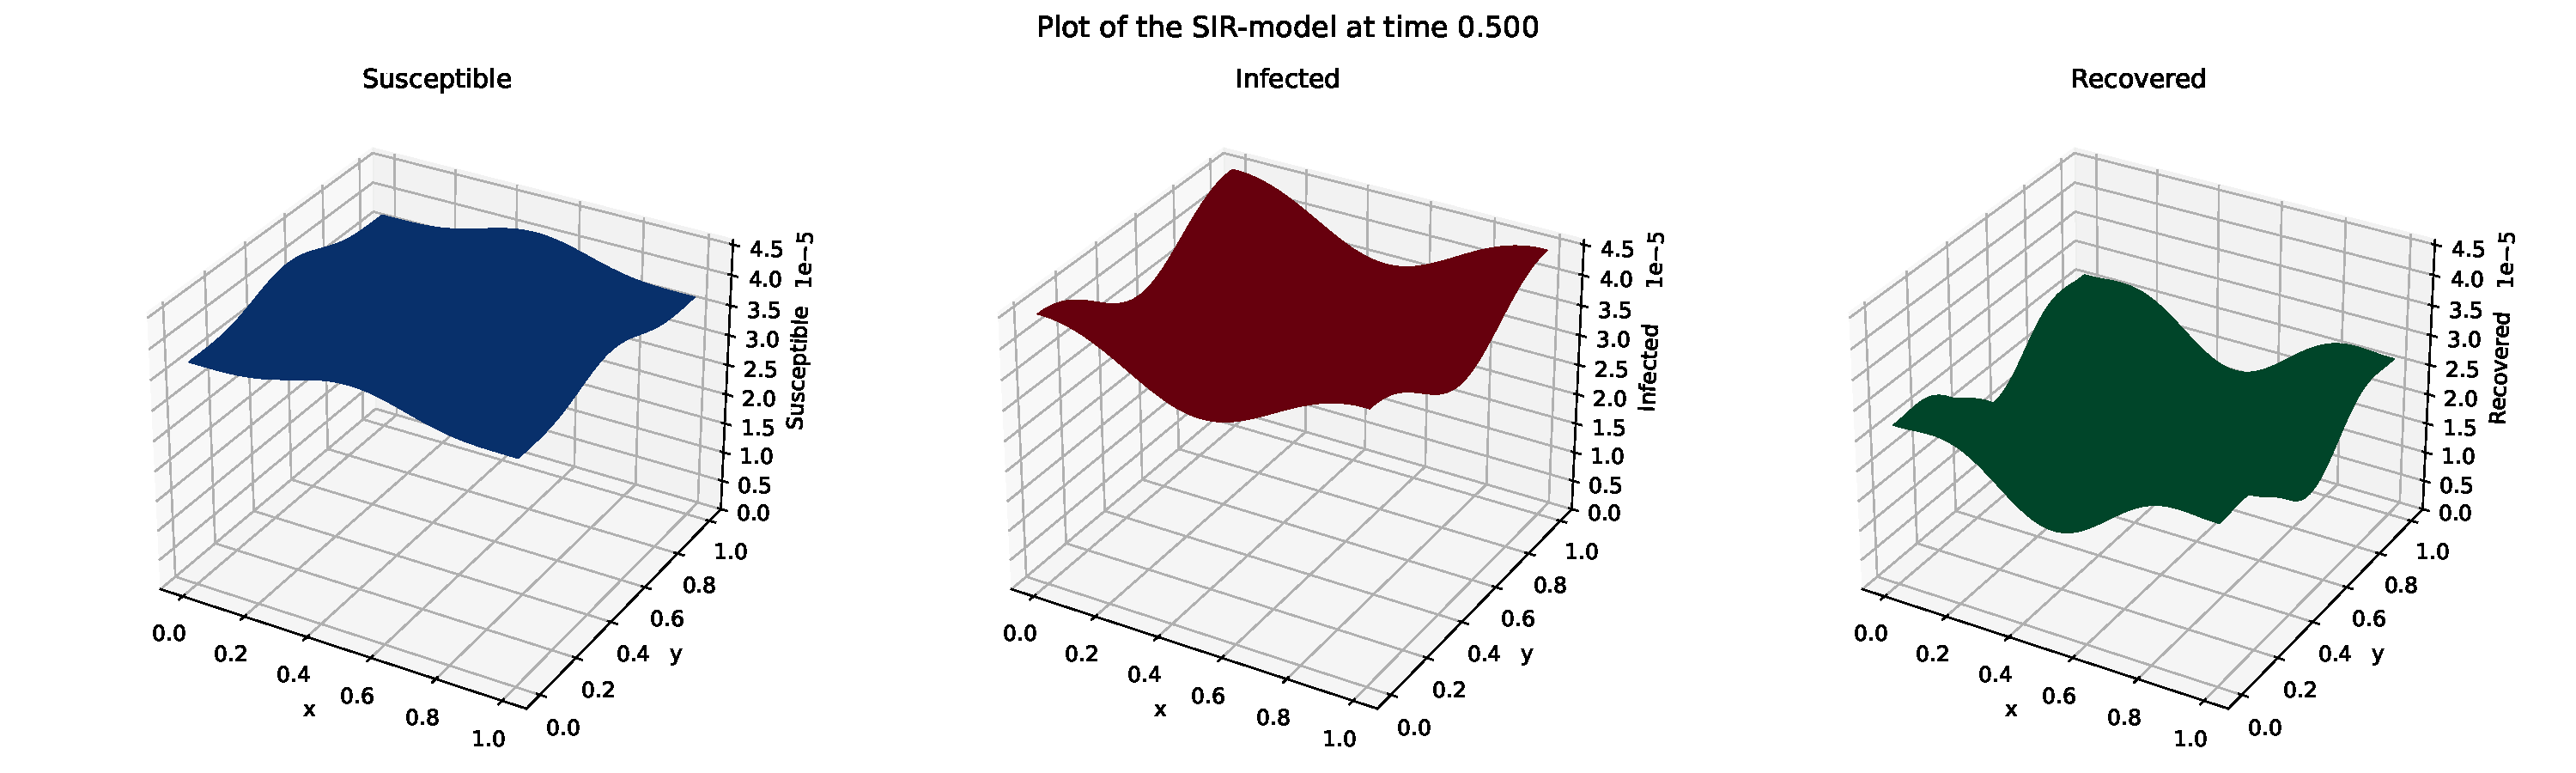
\includegraphics[width=\textwidth]{report/Images/plots/plot-i_t=5000.pdf}
    \caption{Caption}
    \label{fig:enter-label}
\end{figure}

(plot from one square over time)

(plot of population deviation from 1)

The size of the domain influences the parameter choices. The larger domain, the larger the step size in that domain in order to get the same runtime, but that includes larger errors.
In addition the small stepsize, the larger the constants such as $\beta$ needs to be in order to get the same results.


% TODOS: forskjeller i befolkningstetthet, endringer i beta